\subsection{Spectroscopy}

\subsubsection{Raman Spectroscopy}

During spontaneous Raman spectroscopy, a sample is irradiated with radiation of a single frequency $\omega_l$, and radiation scattered from the sample is recorded. A change in the energy of the scattered photons, $\hbar \omega_\nu$ then corresponds to the energy difference between the lowest and first excited vibrational levels of the molecules the light is incident on. For processes where the lowest vibrational level of the ground electronic state $m$ absorb and re-emit a photon, ending up in the first excited vibrational level of the ground state $n$, the frequency of the re-emitted photon is $\omega_l-\omega_\nu$, corresponding to a Raman Stokes process. Similarly, for a process where the state $n$ absorbs and re-emits a photon, ending up in state $m$, the re-emitted photon has a frequency $\omega_l+\omega_\nu$, corresponding to a Raman Anti-Stokes process.\\

The majority of the incident photons undergo Rayleigh scattering. Furthermore, considering the Boltzmann distribution, we expect a majority of systems at room temperature to be in a non-excited vibrational state. This causes Stokes scattering to be more intense than anti-Stokes scattering. This process produces a very faint signal with only around one in $10^7$ scattered photons undergoing Raman scattering \cite{smith_modern_2019}. Spontaneous Raman scattering therefore requires long acquisition times for signal integration, making this process impractical for time-critical implementations or spatial data acquisition.\\

Using the process above, Raman spectroscopy offers a method for probing changes in the polarisability of molecules, which correspond to changes in the vibrational modes of those molecules. It can therefore only detect molecules where the polarisability tensor $\alpha$ changes between different vibrational modes. It should also be noted that this polarisability is related to the intensity of Raman scattering by equation (\ref{eq:raman_intensity}), where $K$ is a constant, $l$ is the laser power, $\omega$ is the frequency of incident radiation, and $\alpha$ is the polarisability of the electrons in the molecule. Note that in tensor form, the polarisability is related to the dipole of a molecule $\mu$ and the electric field from an incident photon $E$ by $\mu=\alpha E$.\\ 
\begin{equation} 
    \label{eq:raman_intensity} 
    I=Kl\alpha^2 \omega^4
\end{equation}

Raman spectroscopy presents many advantages within biological imaging due to its ability to offer chemical insights into the composition of nucleic acids, proteins and lipids \cite{shen_recent_2021} whilst being less affected by water than infrared methods. It also offers narrow excitation bands, making signals relatively easy to classify, and is capable of producing high-resolution images due to the relatively short wavelengths used \cite{xu_raman_2025}.\\

\begin{figure} 
    \centering
    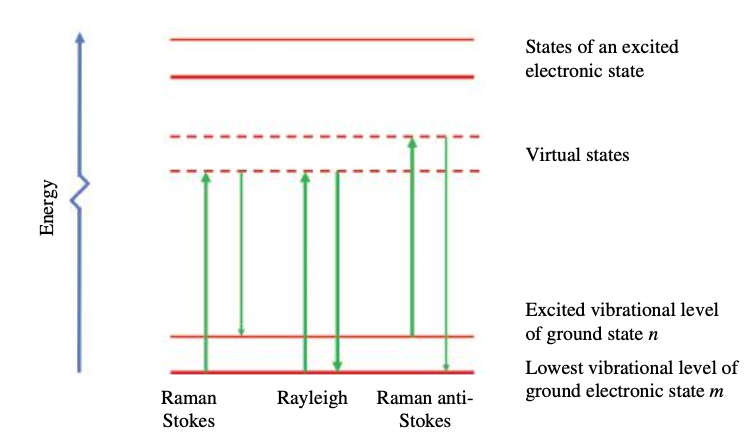
\includegraphics[width=1\linewidth]{Images/raman_energy_levels.png} 
    \caption{The energy levels involved in Raman Stokes and Raman Anti-Stokes processes, from \cite{smith_modern_2019}.} 
    \label{fig:raman_energy_levels} 
\end{figure}

The Raman spectroscopy data for this project has been collected using a patented broadband coherent Raman spectroscopy device, which utilises stimulated Raman spectroscopy (SRS) to pump photons from the excited vibrational level to the ground state, increasing photon emission rates by up to a factor of $10^6$, enabling much faster data acquisition at microscopic resolutions \cite{prince_stimulated_2017}. By using picosecond laser pulses which disperse to have a wide frequency spectrum, it is also possible to conduct these measurements across multiple frequencies simultaneously, further increasing acquisition speed. A basic overview of the CRI system is shown in Figure \ref{fig:CRI_raman}.

\begin{figure} 
    \centering 
    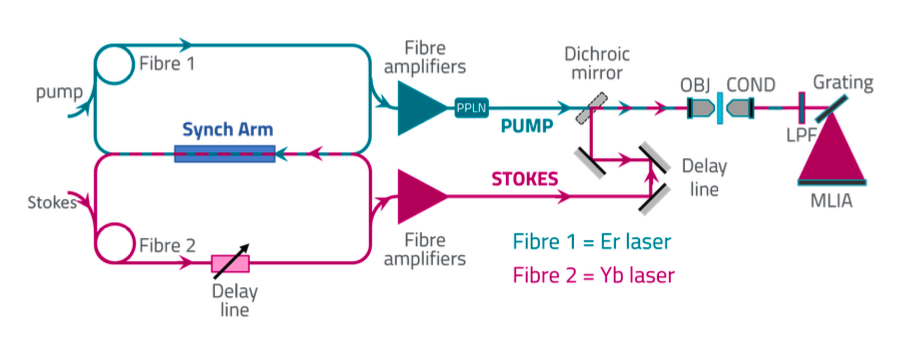
\includegraphics[width=1\linewidth]{Images/cri_raman.png}
    \caption{A schematic overview of the CRI SRS implementation. From CRI.}
    \label{fig:CRI_raman} 
\end{figure}

\subsubsection{Second Harmonic Generation and Two-Photon Excitation Microscopies} The polarisation of a material interacting with light is given by equation (\ref{eq:polarisation}) where $\chi^{(n)}$ is the $n$th order non-linear susceptibility tensor and $\mathbf E$ is the electric field vector \cite{shen_principles_2003}. The second term in equation (\ref{eq:polarisation}) corresponds to second harmonic generation (SHG), whereas the third term corresponds to two- and three-photon absorption and SRS processes.\\

\begin{equation} 
    \label{eq:polarisation} 
    \mathbf{P}(\mathbf{k}, \omega) = \mathbf{P}^{(1)}(\mathbf{k}, \omega) + \mathbf{P}^{(2)}(\mathbf{k}, \omega) + \mathbf{P}^{(3)}(\mathbf{k}, \omega) + \dots 
\end{equation} With 
\begin{align*}
    \mathbf{P}^{(1)}(\mathbf{k}, \omega) &= \chi^{(1)}(\mathbf{k}, \omega) \cdot \mathbf{E}(\mathbf{k}, \omega), \\ \mathbf{P}^{(2)}(\mathbf{k}, \omega) &= \chi^{(2)}(\mathbf{k} = \mathbf{k}_i + \mathbf{k}_j, \, \omega = \omega_i + \omega_j) \\ &\quad : \mathbf{E}(\mathbf{k}_i, \omega_i)\mathbf{E}(\mathbf{k}_j, \omega_j), \\ \mathbf{P}^{(3)}(\mathbf{k}, \omega) &= \chi^{(3)}(\mathbf{k} = \mathbf{k}_i + \mathbf{k}_j + \mathbf{k}_l, \, \omega = \omega_i + \omega_j + \omega_l) \\ &\quad : \mathbf{E}(\mathbf{k}_i, \omega_i)\mathbf{E}(\mathbf{k}_j, \omega_j)\mathbf{E}(\mathbf{k}_l, \omega_l). 
\end{align*}

When incident on a highly polarisable and non-centrosymmetric molecule, two photons can combine upon scattering, causing SHG emission with double the frequency of the incident radiation \cite{perry_two-photon_2012}. Notably, the requirement for non-centrosymmetric environments is a consequence of the second-order symmetry of SHG term in equation (2). As a consequence, incidence on centrosymmetric molecules causes the signal to vanish \cite{chen_second_2012}. This makes SHG especially sensitive to fibrillar collagen in a range of tissues, with changes due to cancerous growths often detectable.\\

The use of two incident photon frequencies from the pump and Stokes beams combined with femptosecond laser pulses for SRS also enable two-photon excitation microscopy to be conducted, where both incident photons simultaneously induce excitations within the incident molecule, which can then be detected \cite{denk_two-photon_1990}. This method is important for cancer detection, as it provides increased imaging depth, can elucidate metabolism within living cells, and can also be conducted using lower energy photons, reducing the risk of photo-damage to a sample \cite{perry_two-photon_2012}. A summary of the energy processes within TPEF and SGH emissions are summarised in Figure \ref{fig:tpef_shg_energies}. 
\begin{figure} 
    \centering
    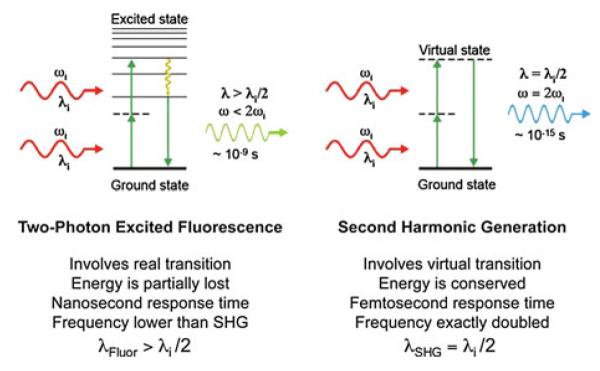
\includegraphics[width=1\linewidth]{Images/nihms-365614-f0001.jpg} 
    \caption{A comparison of the energy processes in TPEF and SHG \cite{perry_two-photon_2012}.} 
    \label{fig:tpef_shg_energies} 
\end{figure}

\subsection{Denoising CHARM Data}
Good progress has also been made in data pre-processing, with members of the CHARM collaboration delivering aligned HE images and pre-processed SRS signals around mid-November. Notably, they used a different pre-processing method for the SRS signal than that detailed in the reports from last year \cite{vali_deep_2024}, \cite{petrov_diagnosing_2024}. It has been noticed in data pre-processing for this work that implementing and expanding on the Fourier domain methods used last year gives similar, but notably different results - see Figure 27. This is therefore an area which warrants further consideration. Potential avenues to explore include using the logarithm of intensity data, as they often cover many orders of magnitude, and taking ratios of SRS channel intensities in an attempt to remove focus-induced systematic errors.

\begin{figure}[h] 
    \centering
    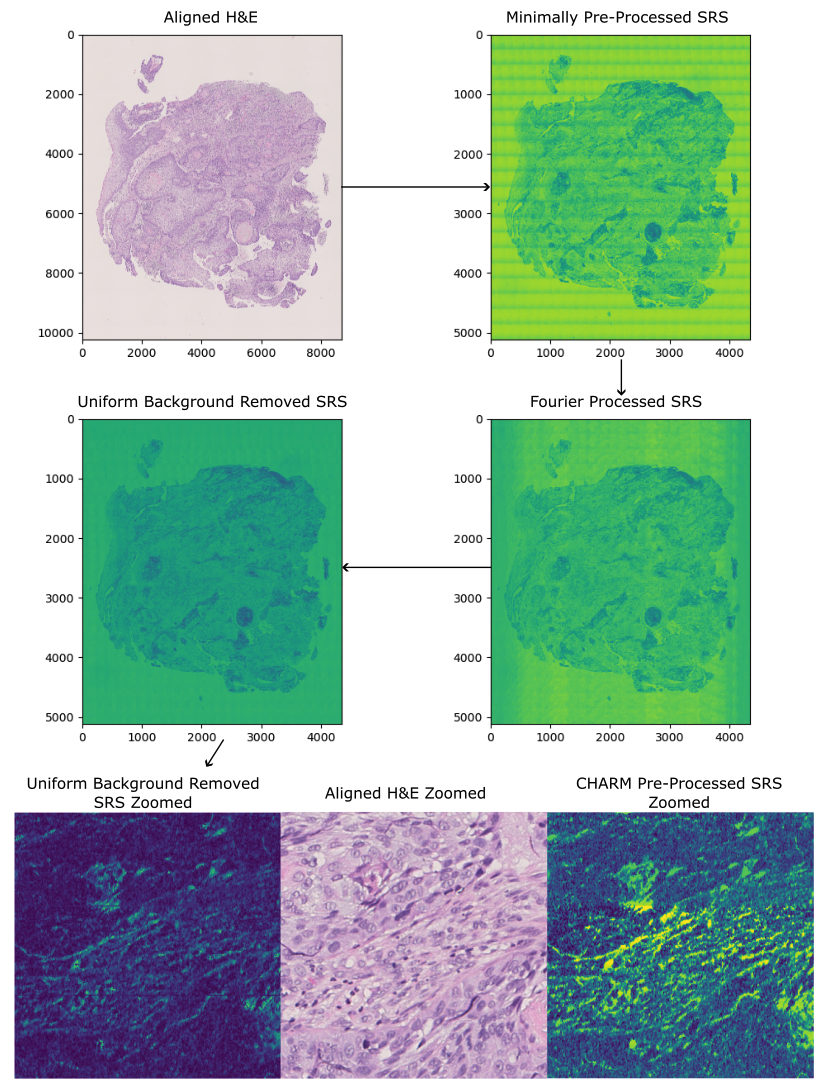
\includegraphics[width=1\linewidth]{Images/different_processing_compare.png}
    \caption{\centering Plots showing a comparison between the Fourier domain noise removal strategy and that used by the CHARM group. The HE images for the respective regions are also provided. Note that the large differences between the SRS signal and the HE image are expected, as we are only showing one of the 31 recorded SRS spectra for the sample.} 
    \label{fig:different_process}
\end{figure}